% !TeX root = ../DistributedConsensus.tex
% !TeX spellcheck = en_GB
\chapter{Reducing Histories to Orders of Execution}
\label{chap:order-of-execution}
\section{Order of Execution}
	A produced combined history represents every action that has occurred on all the events of the workflow.
	It is desired to find an order of execution with excess information in the history removed without losing information regarding the order of the executions. 
	
	\newpar In order to do this, we need to find a single entity denoting an execution, and identify actions that are part of that execution. 
	
	Furthermore, redundant edges between these entities should be removed without losing information about the order of the entities, which corresponds to finding a so-called minimum equivalent graph.
	
	\subsection{Use of the Transitive Closure in Order to Gain Extra Information}
	One approach to finding a single representation of an execution, it could be examined if a single action of the execution could describe all the relations to all the other executions. To do so involves filtering all actions not chosen to be the representative of the execution, and since filtering nodes remove happen before relations, increasing the connectivity of the graph could be beneficial.
	
	It might therefore be possible to establish that two actions have occurred after each other, if each transitive relation in the graph is available on all actions chosen to represent the execution.
	
	\newpar Since the history is represented as a directed acyclic graph, the transitive closure of the graph can be found to find more happens-before relations. 
	After having found the transitive closure of the graph, actions that are either not in between \texttt{Execution start} and \texttt{Execution finish} action types can be filtered away from the graph. One of these execution types should denote an entire execution.
	
	This does not affect the order of the executions, since the execute action types are now connected after having found the transitive closure.
	
	\newpar Finding the transitive closure and filtering does not always give the best possible results however, since actions might appear to happen concurrently after having found the transitive closure, when it is in fact possible to determine that the actions have happened in order. 
	
	\newpar In \autoref{fig:problem:trans} the result of finding the transitive closure of the joined histories of two events is shown. 
	Compare the result to the result of using the \textit{Collapse} approach in \autoref{fig:problem:collapse}, where it can be seen that is is fact possible to determine that these actions happens in order.
	
	\subsubsection{Complexity}
	We implemented finding the transitive closure as a depth first search, which has a running time of $\mathcal{O}(V + E)$. \textit{Collapse} is therefore a more efficient as well as a more precise way of finding an order of execution as described in \autoref{chap:order-of-execution}, and this approach has been determined as the better way of finding the order of execution.\todo[inline]{Igen, mærkeligt at snakke om collapse når denne ikke er defineret endnu.}
	
	\begin{figure}
		\centering
		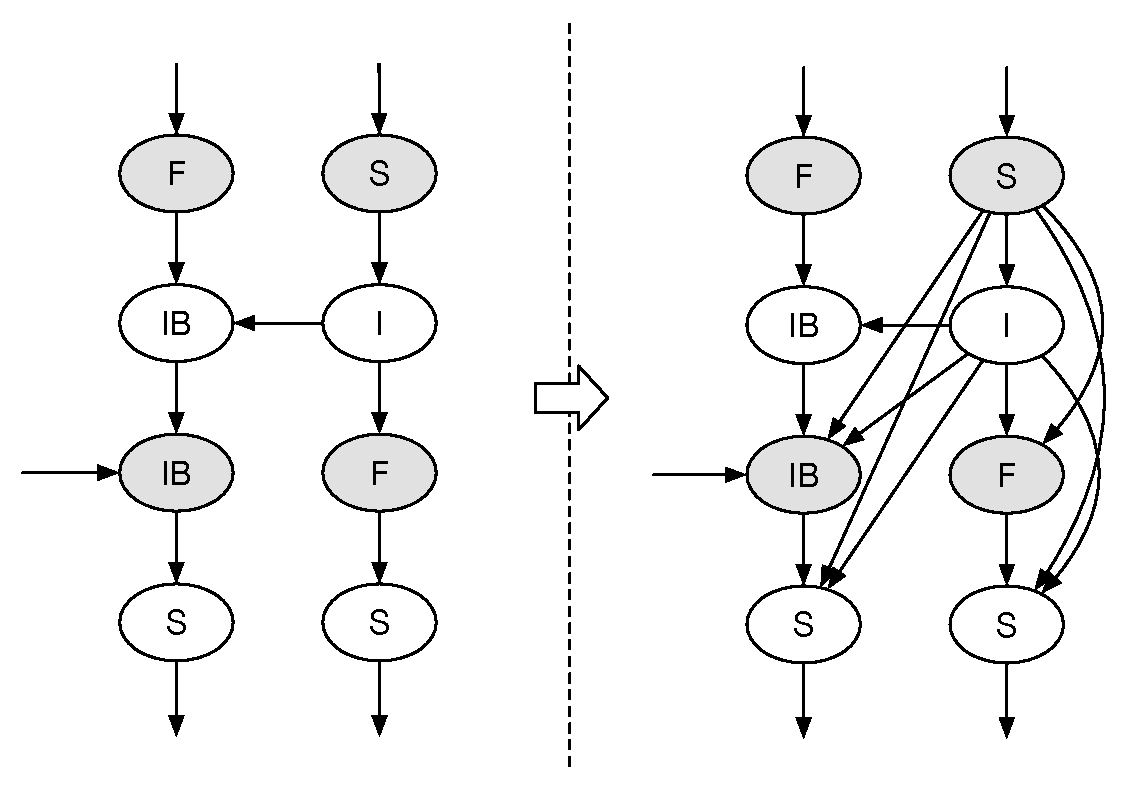
\includegraphics[width=\textwidth]{6orderofexecution/images/trans.pdf}
		\caption{The result of finding the transitive closure on from the actions of an event. Note that the topmost executions happen concurrently. So does the two lower executions.}
		\label{fig:problem:trans}
	\end{figure}
	
	\begin{figure}
		\centering
		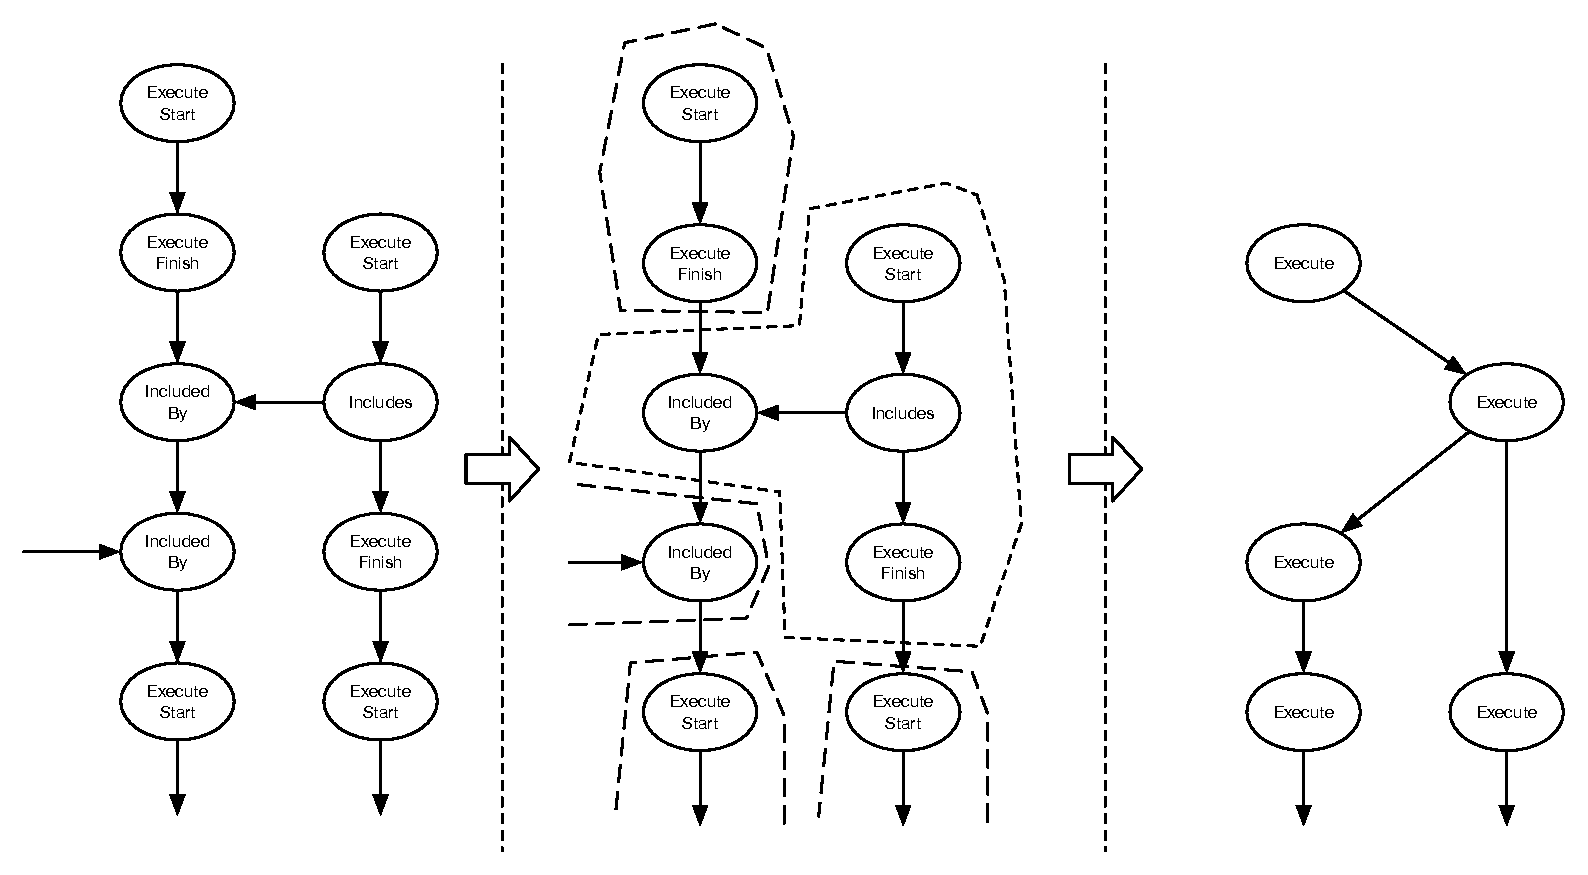
\includegraphics[width=\textwidth]{6orderofexecution/images/collapse.pdf}
		\caption{The result of finding an execution using \textit{Collapse}. Note that executions that previously were concurrent (\autoref{fig:problem:trans}) are now ordered.}
		\label{fig:problem:collapse}
	\end{figure}
	
	\subsection{Collapsing}
	In definition \todo{Lav label til definitions.} we saw that an execution was defined to be all the actions between \texttt{execution start} and \texttt{execution finish} actions. Furthermore even though the receiver \todo{Introduktion til receiver og performer mangler.} saves incoming actions, these actions are still initiated by the performer, and these actions can therefore be seen as being parts of the performers execution. Since an event is only affected by the effects of other events executing or itself, it must be true that any action is always caused by the execution of \textit{some} event, and therefore no action can happened outside any execution.
	
	
	\newpar 
	\todo[inline]{Wat. Forstår overhovedet ikke noget fra her... }
	Due to the property of an execution stated in \autoref{fig:historyinvariant} which states that for an execution, some actions might be concurrent with other actions, while other actions in the execution is able to establish happen before relation to those same actions, it creates complications since executions then happens both concurrent and not concurrently at the same time. 
	\todo[inline]{... til her. Mikael: Enig.}
	
	Because of this problem it is neccesary to formulate a method which is able to \textit{collapse} the execution into a single entity, which has the same happens before relations to actions outside of the execution.
	
	
	To do so it is necessary to make an assumption which states that everything in an execution happens at the same time \todo[inline]{"at the same time" = concurrently? Mikael: Jeg tror simultaneously er bedre?} and therefore any happens-before relation any action has with any action outside of the execution now applies to all events in the execution. When this is the case, every action inside the execution are equal in terms of happens-before relations and therefore we can \textit{collapse} the execution into one single entity. 
	
	The assumption that every action of an execution has the same happens-before relation as any other action in the execution cannot contradict any existing relations, when it is taken into consideration that the events execute serially equivalent. This implies that two executions cannot affect the same event at interpolated\todo{wat? Det skal lige rettes til at beskrive at locking sørger for denne property?} allowing some actions to happen before, and some after, another execution.
	
	\newpar An example of this separation of executions can be found in \autoref{fig:orderofexecution:collapsing}. The figure shows actions that are part of an execution getting collapsed into a single execution, with preserved happens-before relations. 
	
%	\newpar It then is necessary to research a way to \textit{collapse} an execution in order to overcome these problems. \textit{Collapsing} constitutes looking at all actions between an \texttt{ExecuteStart} action and an \texttt{ExecuteFinish} action of an event and connecting these events into a single entity, representing an entire execution. 


%	\newpar When actions contained in an execution have been found, it is necessary to decide what should happen to the grouping of the actions. It is desired to keep all relations intact, to avoid modifying the history and only simplify it. 
	
%	By pointing all ingoing edges to the current event towards a new \textit{collapsed node}, and adding all outgoing edges to the new node, this is accomplished. This new \textit{collapsed node} then represents the entire execution. 

%	In the implemented solution the the \texttt{ExecuteFinish} type has been chosen to denote a collapsed execution in order to avoid creating a new action type. As it can be seen in \autoref{fig:after-collapsing} the collapsing of executions results in an order of execution.

	\begin{figure}[H]
		\centering
		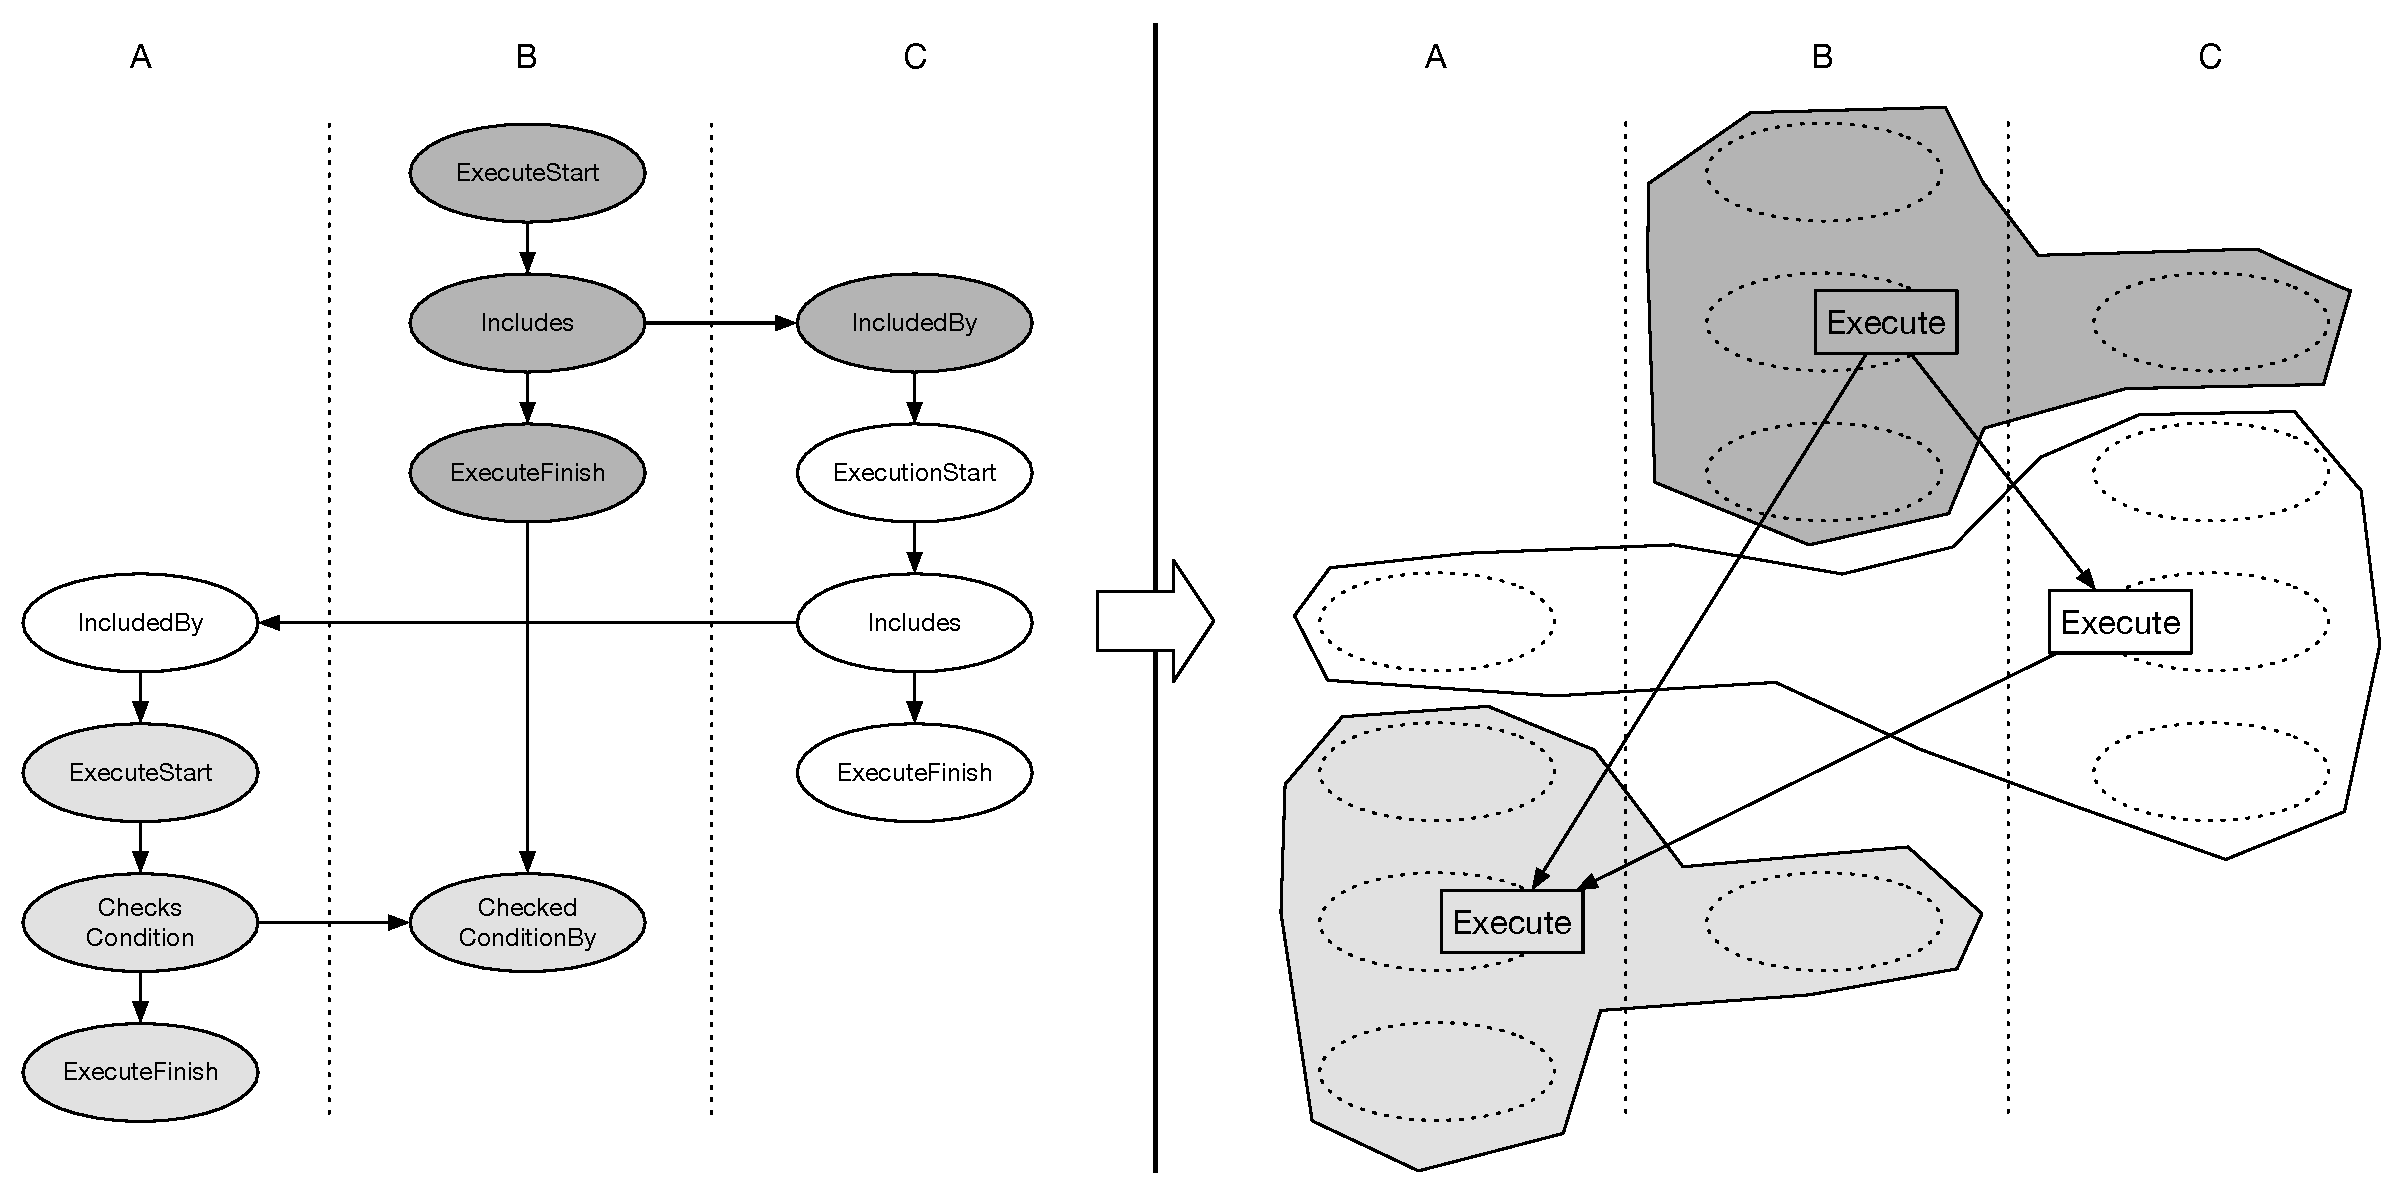
\includegraphics[width=\textwidth]{6orderofexecution/images/transitive-example-collapse.pdf}
		\caption{The result of collapsing actions in the histories of three events.}
		\label{fig:orderofexecution:collapsing}
	\end{figure}
	
%	\begin{figure}
%		\centering
%		\def\svgwidth{0.42\columnwidth}
%		\fontsize{6}{8}\selectfont
%		\import{4connect/images/}{before_collapsing.pdf_tex}
%		\caption{Separation of executions}
%		\label{fig:before-collapsing}
%	\end{figure}
%	\todo{Denne figur skal laves ud fra GasWorkflow.}
%	
%	\todo{udvid (find bedre eksempel) med at særlige tilfælde kræver transitive reduction efter\-følgende}
%	
%%	\begin{figure}
%		\centering
%		\def\svgwidth{0.22\columnwidth}
%		\fontsize{6}{8}\selectfont
%		\import{4connect/images/}{after_collapsing.pdf_tex}
%		\caption{Executions after collapsing}
%		\label{fig:after-collapsing}
%	\end{figure}
%	\todo{Denne figur skal laves ud fra GasWorkflow.}
	
	\newpar The collapsing algorithm can be be seen on \autoref{alg:collapse}. The algorithm gathers all actions of an execution and, after the single entity execution is created, creates all happens-before relations. To argue that the collapse algorithm correctly describes the relations between executions \autoref{fig:historyinvariant} is examined. It states that if there exist any action in execution A with a relation to execution B, then it must not be true the other way around. Therefore for collapse to be correct each single execution entity must have the same property. Since the set of relations the single entity has to other executions is the union of the set of all the actions had to other executions, it must be so that the set cannot contain relations which violates the invariant, because then the invariant would already be broken before the collapse. By proof of contraditction, it it was so that the invariant is broken in the union set, then there is a value where A happens before B and B happens before A, then the original collection of sets must already have had these two relations.
	
	\todo[inline]{Check if you like this argumentation.}
	
	\begin{algorithm}[H]
		\begin{algorithmic}
			\Function{Collapse}{graph}\State
				locals: CollapseMap: Mapping from old to newaction IDs.
				\State\hspace{28pt} Result: Graph, initially empty
				\State
				\State ExecuteStarts $\leftarrow$ \Call{Filter}{type = ExecuteStart, graph} \State
				Executions $\leftarrow$ \Call{Map.map}{FindSingleExecution, ExecuteStarts}
				\ForAll{executions in Executions}\State
					CollapseMap $\leftarrow$ \Call{CreateExecutionMap}{execution, newExecutionId, CollapseMap}
				\EndFor
				\ForAll{oldActionID, newActionID in CollapseMap}
					\State
					NewAction $\leftarrow$ Action with \State\hspace{28pt}ID = newActionID and \State\hspace{28pt}Edges = edges from oldActionID in graph mapped to new IDs\State
					Result $\leftarrow$ \Call{AddNode}{NewAction, Result} \State\Comment{This requires AddNode to merge edge sets when existing nodes are added}
				\EndFor
				
			\EndFunction
			\State
			\Function{FindSingleExecution}{startAction}
				\State locals: execution
				\While{startAction.Type $\neq$ ExecuteFinish} \State
					execution $\leftarrow$ \Call{AddRange}{startAction.Edges, execution}
				\EndWhile\State
				\Return execution
			\EndFunction
			\State
			\Function{CreateExecutionMap}{ActionSet, newActionId, accumulatorMap}
				\ForAll{actions in ActionSet}\State
					accumulatorMap $\leftarrow$ \Call{Add}{action.Id, newActionId, accumulatorMap}
				\EndFor \State
				\Return accumulatorMap
			\EndFunction
		\end{algorithmic}
		\caption{Collapse algorithm}
		\label{alg:collapse}
	\end{algorithm}
	
	\newpar The algorithm runs in a time complexity of $O(n^2)$ where $n$ is the number of actions in the history. This must be so since $CreateExecution$ runs linearly in $n$ if $Add$ on $map$ is constant and $CreateExecution$ worst case gets called $n/2$ times if every action in the history are executions. \todo{write better more correct yes}
	
	\subsection{Transitive Reduction}
	
	\newpar Redundant edges might still exist in the history after executions of the history have been collapsed, as seen in \autoref{fig:orderofexecution:collapsing}. An edge is redundant in cases where there exists a non-direct path from an execution to another execution, but there also exists a direct edge between the two executions. In this case the direct edge is redundant and can be removed, since it does not contribute extra information in regards to the ordering of the executions as it only explicitly expresses what is implicitly available. Removing it will not affect the ordering or reachability of the order of execution, but rather simplify the order of execution.
	
	\newpar An example of a redundant edge in a collapsed order of execution can be seen in figure \autoref{fig:orderofexecution:collapsing}. The figure illustrates a case where a redundant edge exists between event $A$ and event $B$, since the edge from event $B$ through $C$ provides more information about the order in which the executions occurred. 
	Recall that the order of execution is represented as a directed acyclic graph and that it is possible to find a minimal equivalent graph for such a graph. 
	
	\newpar In directed acyclic graphs the transitive reduction of a given graph is a graph with the fewest possible number of edges, but the same reachability as the given graph.	That is, if there exists a path from an edge $x$ to an edge $y$ in graph G, there must also be a path from $x$ to $y$ in the transitive reduction of $G$, and vice versa.
		
	Furthermore, the transitive reduction will always be a subgraph of the given graph. For that reason the transitive reduction corresponds to the minimum equivalent graph.\todo[inline]{Jeg (Mikael) har det lidt med subgraph som jeg har det med subset. Jeg er ikke helt sikker på hvad det betyder i denne sammenhæng - Altså, jeg synes ikke det hjælper til min forståelse af problemet (hvilket jeg i øvrigt synes er udpenslet nok på dette tidspunkt.)}
	
	The implementation for finding the transitive reduction on an order of execution is shown in \autoref{alg:orderofexecution:reduction}.
	
	\begin{algorithm}[H]
		\begin{algorithmic}
			\Function{Transitive-Reduction}{$history$}
				\ForAll{$execution1$ \textbf{in} $history$}
					\ForAll{$execution2$ \textbf{in} $history$}
						\If{\Call{pathExists}{$execution1$, $execution2$, $history$}}
							\ForAll{$execution3$ \textbf{in} $history$}
								\If{\Call{edgeExists}{$execution2$, $execution3$, $history$}}
									\If{\Call{edgeExists}{$execution1$, $execution3$, $history$}}
										\State $history$ $\leftarrow$ \Call{removeEdge} {$execution1$, $execution3$, $history$}
									\EndIf
								\EndIf
							\EndFor
						\EndIf
					\EndFor
				\EndFor
			\State
			\Return $history$
			\EndFunction
		\end{algorithmic}
		\caption{Transitive Reduction Algorithm}
		\label{alg:orderofexecution:reduction}
	\end{algorithm}
	
	\newpar The shown algorithm for transitive reduction has a time complexity of $O(n^3)$ where $n$ is the number of executions, since the algorithm has three nested for-loops over all executions in the history. This is based on the requirements that $pathExist$ runs in linear time and $edgeExist$ is a constant lookup. In actual use cases the graph will not be totally connected and therefore the innermost loop will not be executed for most executions. \todo{check if pathExists runs linearly}
	
	\begin{figure}[H]
		\centering
		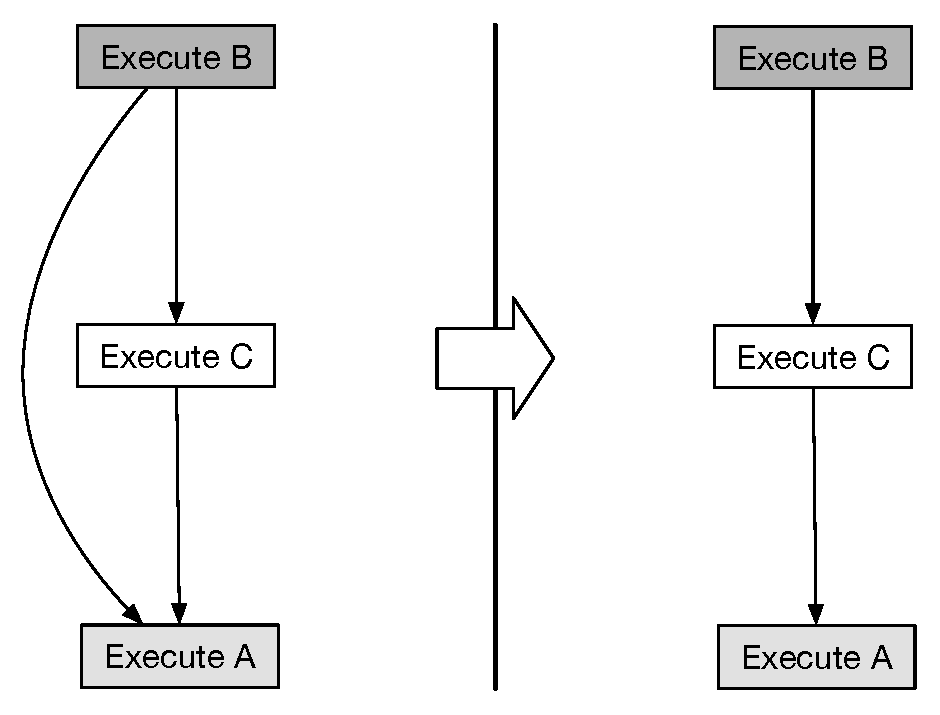
\includegraphics[height=0.35\textheight]{6orderofexecution/images/reduce-before-after.pdf}
		\caption{The result of reducing an order of execution with redundant edges.}
		\label{fig:orderofexecution:reduce-before-after}
	\end{figure}

% Synes ikke det hører til her	
%	\newpar These algorithms do not provide a way to ensure that malicious nodes cannot tamper with the history. As in the case where one event represented the workflow, there is no way of making sure that the event creating the history will not tamper with the history. It would be possible to pinpoint which neighbouring events are malicious if enough of the neighbours have relations to each other. 


	\section{Election} 
	As we have now found an order of execution where (potentially) malicious events have been identified, we want to know if the remaining events can agree upon the rest of order of execution.
	
	\newpar As stated in the problem definition, it is desired to reach consensus on the resulting order of execution, but since no process in the system knows the entire state of a workflow, it is not possible for the events to suggest an order of execution without completing steps alike with the ones described in this report.
	
	\newpar Because we have chosen to let the client know all events in order to retrieve their histories, it is also easy for us to send the resulting order of execution back to them, in order to find out whether or not they can agree to this order.
	
	\newpar When any event receives this order of execution, it can look at its own history and at the received order. The local history can contain executions with outgoing actions between execute start and execute finish actions. Furthermore ingoing relations can be identified as executions of other events from the following rules:
	
	\begin{itemize}
		\item Each counterpart present in actions with ingoing action types must have executed at least once, in order to contact the local event.
		\item If two actions with the same ingoing action type and counterpart are present after each other, this denotes two separate executions of the counterpart event, because each executing event only contacts another event once per relation when executing.
	\end{itemize}
	
	%\newpar Furthermore if an event has sent multiple ingoing requests as part of a single execution, then each of the relations that these actions represent must be present every time that execution has happened.
	%Ovenstående er udkommenteret fordi det relaterer mere til validation end election.
	
	\newpar	Given these rules, the local history can be turned into a "local order of execution".
	\figuretodo{Tilføj figur der viser hvordan en lokal historik kan omdannes til en order of execution der kan bruges til afstemning.}
	
	\newpar Now that the event has created a local order of execution, this order can be used to decide whether or not the event can agree on the global order of execution. If there exists a path from one execution to another in the local order of execution, there must also exist a path between these executions in the global order of execution for the event to agree. Because the local history is totally ordered, the local order of execution must also be totally ordered.\todo[inline]{proof?}
	
	With this property the event can find the local order of execution in the global order. \todo[inline]{The following algorithm assumes that an execution can be found across local and global orders of execution.}Algorithm \ref{alg:vote} outlines how this can be done.
	
	\begin{algorithm}
		\begin{algorithmic}
			\Function{Vote}{localHistory, globalOrderOfExecution}
				\State\hspace{2em}\textbf{returns} \texttt{True} if the paths between executions in the local history are present in the
				\State\hspace{6em}global history. \texttt{False} otherwise.
				\State localOrderOfExecution $\leftarrow$ \Call{MakeLocalOrderOfExecution}{localHistory}
				\State localExecution $\leftarrow$ execution in localHistory with lowest local timestamp
				\While{\Call{IsNotNull}{currentLocalExecution}}
					\If{\Call{IsEmpty}{currentLocalExecution.Edges}}
						\State \Return \texttt{True}
					\EndIf
					\State globalExecution $\leftarrow$ find localExecution in globalOrderOfExecution
					\State nextGlobalExecution $\leftarrow$ find next local execution in globalOrderOfExecution
					\If{\Call{HasPath}{globalExecution, nextGlobalExecution, globalOrderOfExecution}}
						\State\Return \texttt{False}
					\EndIf
					
					\State localExecution $\leftarrow$ \Call{SingleOrNull}{localExecution.Edges}
				\EndWhile
			\EndFunction
		\end{algorithmic}
		\caption{The \textit{\textbf{Vote}} algorithm}
		\label{alg:vote}
	\end{algorithm}
	
	If the history is correct, and the nodes are correct, then the nodes will vote in favour of the history.
	
	It is possible to decide a threshold for the ratio between the number of good nodes and the number of malicious nodes. If the result of the election is better than the threshold, then distributed consensus between the nodes exists for the history. In distributed systems this threshold is normally set to the majority of the participating nodes, which means at least one more than half the amount of nodes.\todo[inline]{Find a source.}
	
	\newpar Election is not an actual vote on the result of the resulting order of execution. Election is instead a confirmation that the algorithm has produced the correct result. \todo[inline]{Giver det her stadig mening?}
	
	\todo[inline]{Tilføj correctness proof/paragraph. "There should be a theorem or something clearly stating that this algorithm solves the original problem."}
	\figuretodo{Tilføj figur: Kan vi på nogen måde vise resultatet af election?}